
%%!TEX root = ./heapvis.tex

\begin{figure*}[t]
  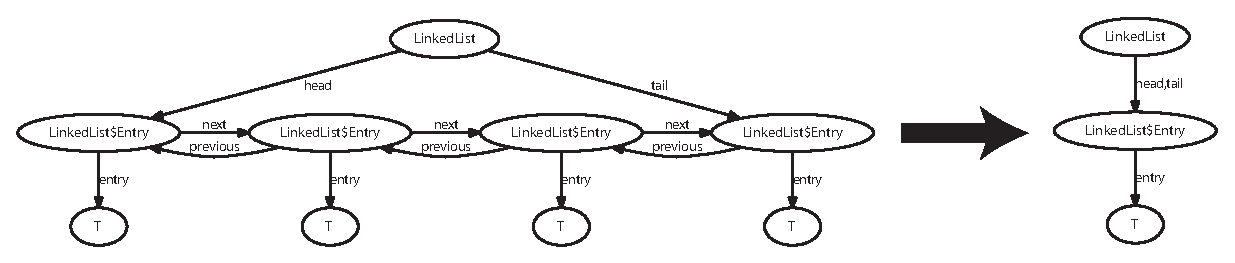
\includegraphics[width=\textwidth]{figs/linked-list-both}
  \caption{An example of applying our summarization algorithm to a linked
list.  Our algorithm first summarizes all \texttt{LinkedList\$Entry} objects
into a single node, then summarizes all \texttt{T} objects into a single
node.  Note that the summary would look the same regardless of the number of
\texttt{T} objects in the linked list.}
  \label{fig:linked-list}
\end{figure*}


\section{Heap Analysis}
\label{analysis}

\subsection{Heap Snapshot}

Our heap analysis starts with a heap snapshot obtained from a running Java
program.  The heap snapshot tells us which objects are currently in the heap,
what their field values are, including the pointer values, and the values of
all root references (static variables and stack references).  In addition, the
heap snapshot provides the runtime type of each object instance and the number
of bytes needed to represent each object.

We use Sun's HPROF tool~\cite{hprof} to generate heap snapshots. HPROF is an
agent that connects to a host Java virtual machine and uses the JVM Tool
Interface~\cite{jvmti} to enumerate all the objects in the program's heap. 
HPROF outputs the snapshot in a
well-documented binary format that is supported by many third-party profiling
and memory analysis tools.  HPROF runs on top of any JVM that supports the JVM
Tool Interface, so it is independent of JVM implementation.
%\todo{AG: This is a bit redundant since you've just said so in the previous section.}

One of our goals is to allow the programmer to view the heap at any point in
the program's execution. To support this capability we provide a
mechanism for dumping a heap snapshot from within the program itself.  Since the
source to HPROF is provided with the Java Development Kit, we modify it to
include a class \texttt{Dumper} with a static method \texttt{dumpHeap()} that
generates the heap snapshot when called. The programmer adds a call to
\texttt{dumpHeap()} in the source code at the point where a heap visualization
is desired.

% SZG: not really analogous to debugger...
%Thus the user can insert a call to this method into the target code to produce 
%a heap snapshot, similar to setting a breakpoint in a debugger.

%HPROF outputs the heap snapshot in a well-defined binary format, which
%our heap analyzer then can parse.
%\todo{AG: Could the user insert multiple dumpHeap() calls in a program?
%Could the user dynamically call this method while running a program? I.e. not is there a way to call it from outside, but more can dumpHeap be called at runtime?}

\subsection{Heap Analyzer}

\subsubsection{Input Format}

Our heap analyzer takes the heap snapshot from HPROF and parses it into
a sequence of records.  Of interest are the class records, which tell us
details about the types of the objects in the heap snapshot, the object 
instance records, which give the types of these objects and their field values,
and the root records, which tell us which heap objects are pointed to by
root pointers (stack references and static references).  Using these data,
the heap analyzer builds a graph representation of the program heap, mapping
object instances to graph vertices, pointer fields to graph edges, and roots
to entry points in the graph.  

\subsubsection{Summarization Algorithm}

Typical Java programs may contain 100,000, 1,000,000, or more live objects at any 
given point in program execution~\cite{blackburn06dacapo}; drawing
all these objects would make the visualization too cluttered to comprehend 
and too slow to interact with.  Our heap analyzer \emph{summarizes} 
the graph to make visualization manageable.  

Our summarization algorithm is designed to reduce the size of the graph 
while retaining the relationship among nodes.  Each node in the summary graph
represents a set of nodes in the concrete graph with the same runtime type 
and similar connectivity, and the edges in the summary graph represent
sets of edges in the concrete graph.  It works by merging nodes in the 
concrete graph according to a set of rules, and repeatedly applying those
rules until it reaches a fixed point.

The rules for merging are:
\begin{enumerate}
\item \textbf{If there exists a reference from object $o_1$ to object $o_2$, 
and $o_1$ and $o_2$ are of the same type, merge $o_1$ and $o_2$.} This rule
merges the recursive backbone of a data structure (e.g. the nodes of a 
linked list or the nodes in a tree).
\item \textbf{If objects $o_1$ and $o_2$ have the same set of predecessor 
objects (objects that point to $o_1$ or $o_2$) and are of the same type, 
merge $o_1$ and $o_2$.}
This rule merges sets of objects that have the same type and the same
connectivity (e.g. the objects contained by a data structure).
\end{enumerate}

With these two simple rules, our system can compress very large graphs into
more manageable ones.  Consider the linked list data structure of
Figure~\ref{fig:linked-list}.  This linked list contains four objects of type
\texttt{T}.  Our summarization algorithm first merges all the
\texttt{LinkedList\$Entry} objects into a single object using rule 1, and then
all the \texttt{T} objects into a single object using rule 2.   Note that the
summarized graph looks the same no matter how many elements the linked list
contains --- whether 4, 400, or 40,000.  However, if the linked list contains
objects of different types, the summarized graph will contain separate nodes
for the set of objects of each type.  

%\todo{AG: Is there any way to identify
%which objects are merged ones? Would it be useful? Would it be useful to know
%how many objects got merged into one?  -- OK, partially, answered by 5.2}

\subsubsection{Output Format}

We write the summarized graph in GraphML format~\cite{graphml} for the 
heap visualizer to import and display.

